\documentclass{article}
\usepackage[utf8]{ctex}
\usepackage{lineno,hyperref, tablefootnote, booktabs, graphicx,  subfigure, amsmath}
\usepackage[margin=1in]{geometry} %页边距
\title{信号处理原理实验}
\author{张晨}
\begin{document}

\maketitle

\section{双音频按键识别}
\subsection{实验原理}
电话拨号时,按下每个键会发出不同的声音,这是因为每个按键的声音包括两个不同频率的正弦信号。将时域上的声音信号转变到频域上,即可提取出这两个正弦信号,从而识别出按下的按键。

将时域信号变为频域信号的常见做法有以下两个:
\begin{enumerate}
    \item FFT,以$O(n\log n)$的时间复杂度求出各个频率的分量大小。
    \item Goertzel,以$O(n)$的时间复杂度求出某一个频率的分量大小。
\end{enumerate}
实验说明中给出了Goertazl算法的原理式。

\begin{equation}
\begin{aligned}
&v_{k}(n)=x(n)+2 \cos \left(\frac{2 \pi k}{N}\right) v_{k}(n-1)-v_{k}(n-2)\\
&y_{k}(n)=v_{k}(n)-v_{k}(n-1) W_{N}^{k}\\
&v_{k}(-1)=v_{k}(-2)=0
\end{aligned}
\end{equation}
其中,第二个式子可进一步化简为
\begin{equation}
    y_{k}(n) * y^*_{k}(n)=v_k(n-1)^2 + v_{k}(n)^2 - 2\cos \left(\frac{2 \pi k}{N}\right) v_{k}(n-1) v_k(n)
\end{equation}

具体实现时,将音频信号切分成若干小段,分别在频域上进行分析提取出按键,最后再进行去重。

\subsection{实验结果}
我使用了两个测例进行测试。一个是录下的$123456789*0\#$,下称手机音频,另一个是从B站获取的使用按键演奏欢乐颂的片段,下称欢乐颂。程序输出如图\ref{fig:1-output}所示。
\begin{figure}
    \centering
    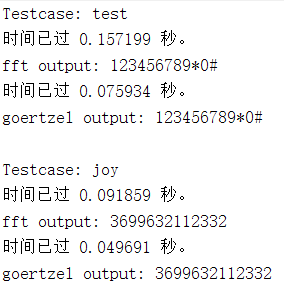
\includegraphics[width = 0.3\textwidth]{problem1/output.png}
    \caption{实验1程序输出}
    \label{fig:1-output}
\end{figure}
\subsubsection{准确性}
这两个算法均能准确识别出按键音,但是欢乐颂中存在多次快速按下同一个键的情况,暂未找到分开这些按键音的方法。识别的效果如图\ref{fig:1-acc}所示。
\begin{figure}[htbp]
\centering
\subfigure[手机音频,FFT]{
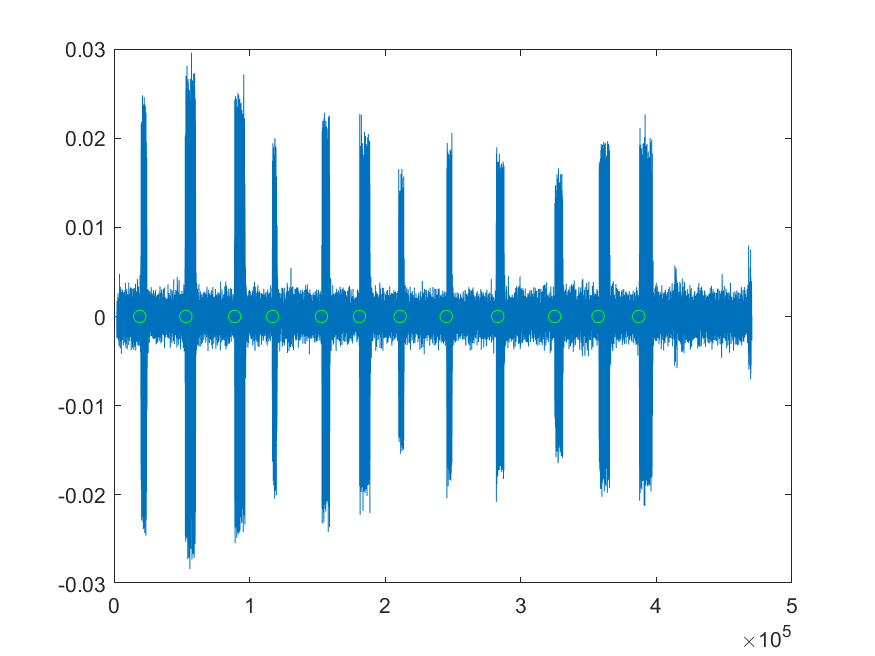
\includegraphics[width = 0.22\textwidth]{problem1/test-fft.png}
\label{fig:test-fft}
}
\subfigure[手机音频,Goertzel]{
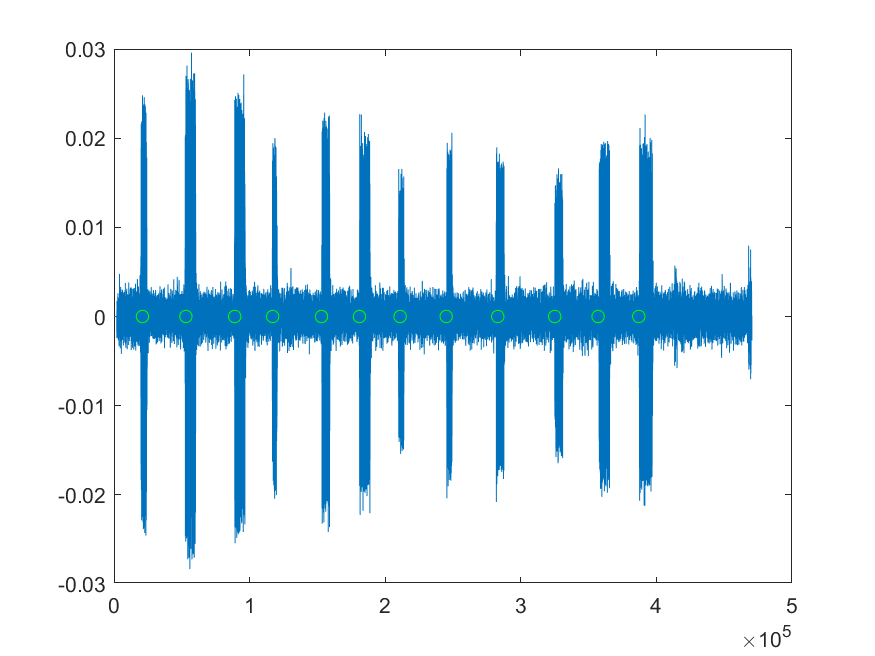
\includegraphics[width = 0.22\textwidth]{problem1/test-goertezl.png}
\label{fig:test-goe}
}
\subfigure[欢乐颂,FFT]{
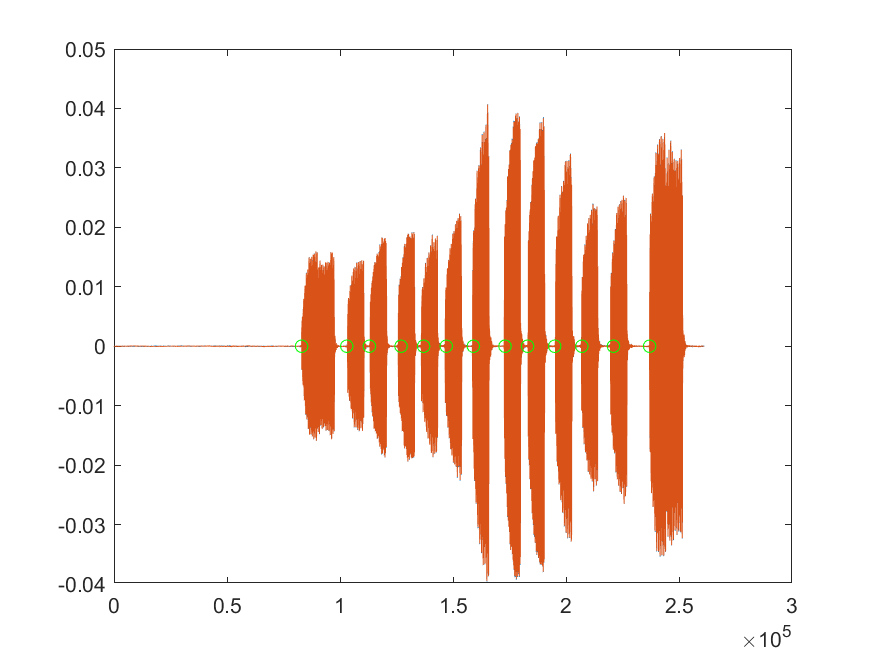
\includegraphics[width = 0.22\textwidth]{problem1/joy-fft.png}
\label{fig:joy-fft}
}
\subfigure[欢乐颂,Goertzel]{
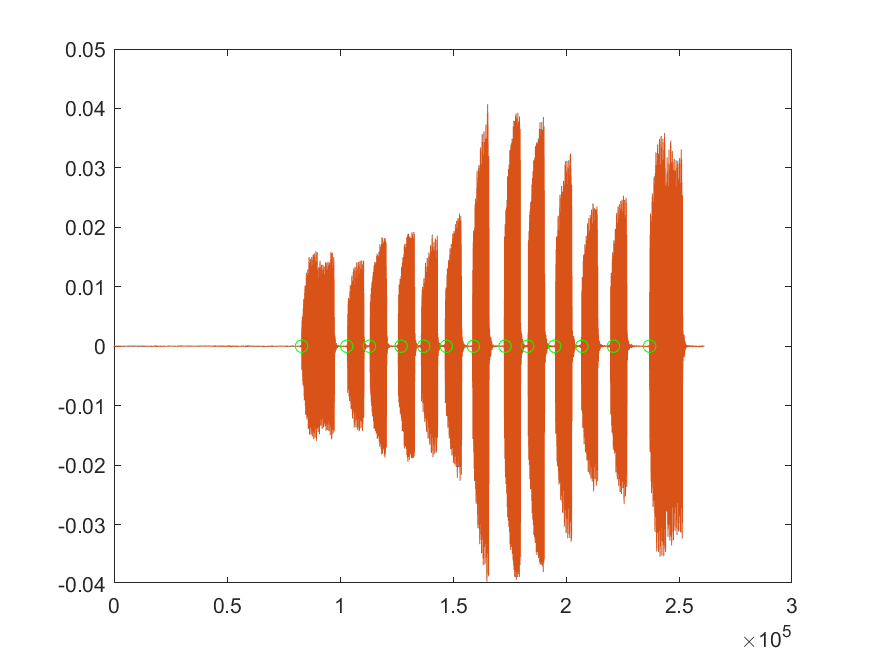
\includegraphics[width = 0.22\textwidth]{problem1/joy-goertezl.png}
\label{fig:joy-goe}
}
\caption{按键识别情况,识别出的按键以圆圈标出。}
\label{fig:1-acc}
\end{figure}
\subsubsection{运行效率}
两算法的效率对比如表\ref{tab:1-eff}所示。可以看出,Goertzel的速度大致是FFT的两倍。
\begin{table}[htbp]
\centering
\begin{tabular}{|l|l|l|} \hline
    & FFT & Goertzel \\ \hline
    手机音频 & 0.157199 秒 & 0.075934 秒 \\ \hline
    欢乐颂 & 0.091859 秒 & 0.049691 秒 \\ \hline
\end{tabular}
\caption{两种算法的运行效率对比}
\label{tab:1-eff}
\end{table}
\section{卷积计算方法的性能比较}
\subsection{实验原理}
总计实现了以下4种卷积计算方法
\begin{enumerate}
    \item 直接计算法 直接套用卷积的公式
    \item 圆卷积法 $y(n) = x(n) * h(n) = IDFT[DFT(x) \cdot DFT(h)]$,为使用快速傅里叶变换加速,应将序列补齐至长度为2的整数次幂。
    \item Overlap Add 将序列$x$拆分成若干段,每段分别计算与$h(n)$的卷积,最后再累加起来。
    \item Overlap Save
    将结果序列拆分成若干段,分别进行计算。
\end{enumerate}
\subsection{实验结果}
Overlap Add 和 Overlap Save的运行时间与切分长度有密切的关系。通过实验,我发现在Overlap Add中,切分长度取3倍$h(n)$的长度左右比较合适,Overlap Save则需要取到9倍$h(n)$的长度左右。以下实验都基于这组参数。
\subsubsection{直接计算法与其他方法}
实验结果如图\ref{fig:bf}所示。可以发现,直接计算法(bruteforce)明显慢于其他的做法。这是因为其时间复杂度为$O(n^2)$,而其他做法的复杂度都为$O(nlogn)$。
\begin{figure}[htbp]
    \centering
    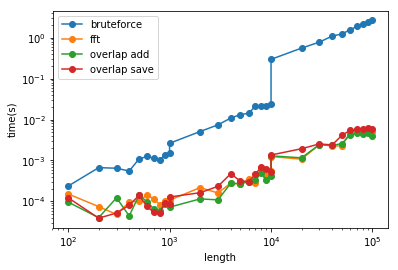
\includegraphics[width = .7\textwidth]{problem2/time_all.png}
    \caption{四种方法的运行时间比较。横坐标为x的长度。x长100至900时,h长100;x长1000-9000时,h长1000;x长10000至90000时,h长10000。坐标皆为对数坐标。}
    \label{fig:bf}
\end{figure}
\subsubsection{Overlap的效果}
从图\ref{fig:overlap}中可以发现,只有在两序列长度相差悬殊的时候,overlap才会起到作用。Overlap Add的性能要好于Overlap Save,这是因为Overlap Add引入的冗余计算仅仅为若干次加法运算,而Overlap Save却引入了更多的傅里叶变换的计算。
\begin{figure}[htbp]
\centering
\subfigure[len(h(n))=100]{
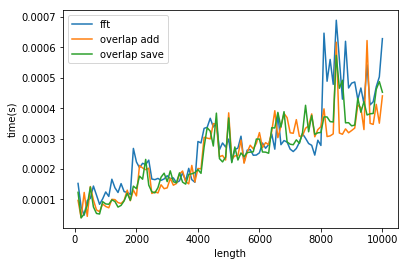
\includegraphics[width = 0.3\textwidth]{problem2/100.png}
}
\subfigure[len(h(n))=1000]{
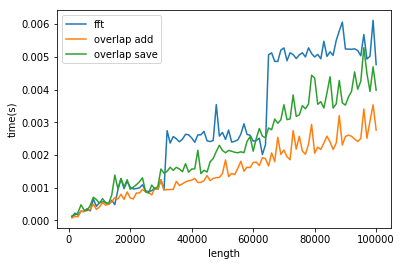
\includegraphics[width = 0.3\textwidth]{problem2/1000.png}
}
\subfigure[len(h(n))=10000]{
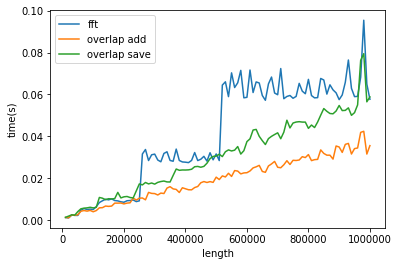
\includegraphics[width = 0.3\textwidth]{problem2/10000.png}
}
\caption{两种Overlap方法与圆卷积法的运行时间对比,横坐标为x(n)的长度。}
\label{fig:overlap}
\end{figure}

\section{语音信号的频分复用}
\subsection{实验原理}
语音主要分布在一个很狭小的频带里,因此可以将多个语音信号在频域上依次排开,达到频分复用的效果。
\subsection{实验结果}
我从新闻联播上录了三段音频,它们的原始时域信号如图\ref{fig:input-time}所示。
\begin{figure}[htbp]
\centering
\subfigure{
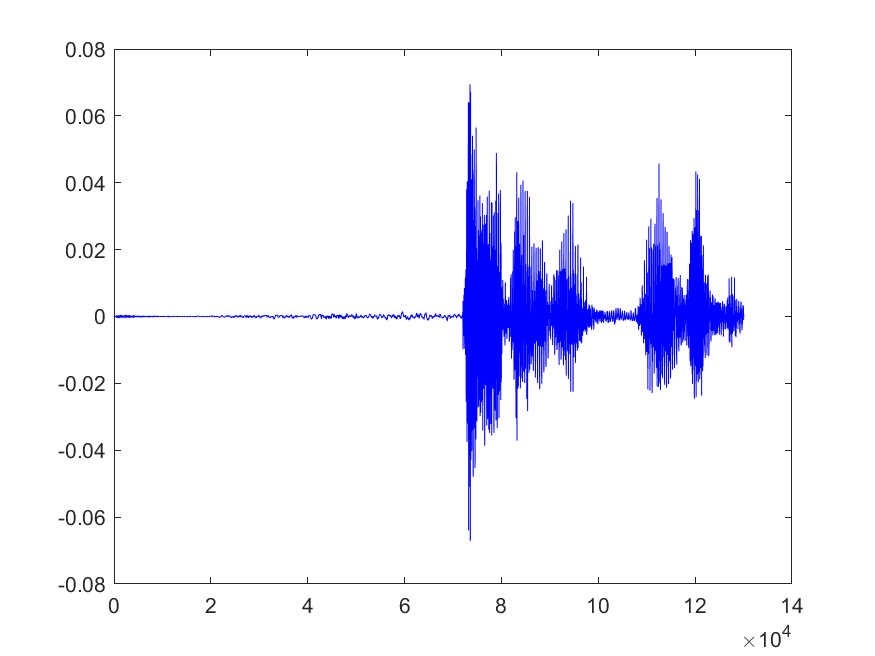
\includegraphics[width = 0.3\textwidth]{problem3/input-time-Recording1.png}
}
\subfigure{
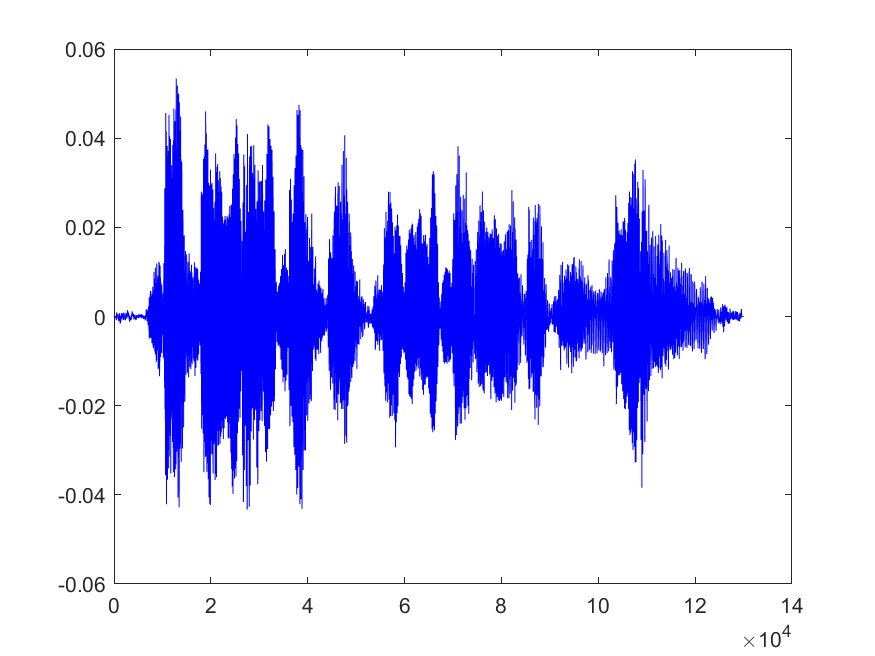
\includegraphics[width = 0.3\textwidth]{problem3/input-time-Recording2.png}
}
\subfigure{
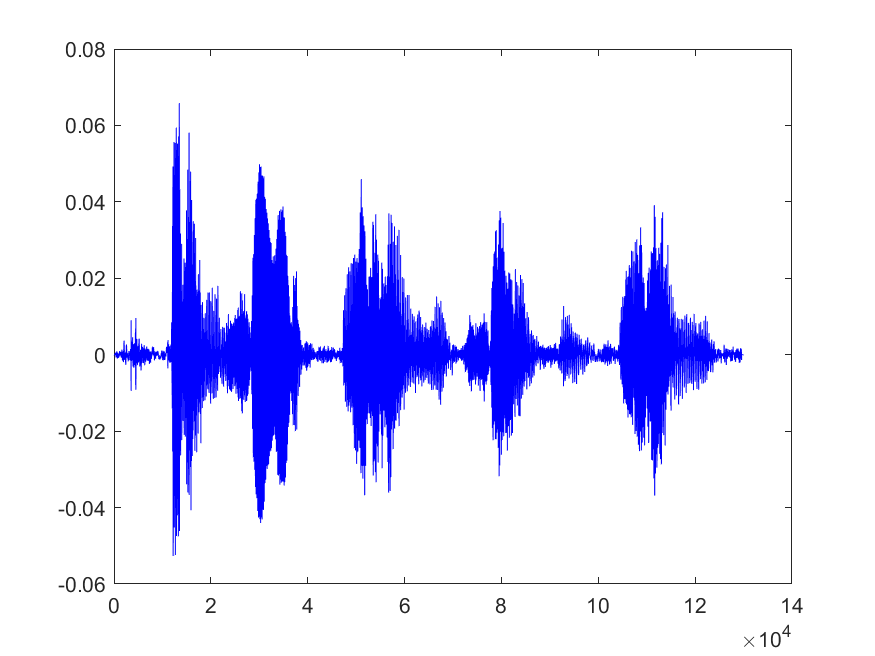
\includegraphics[width = 0.3\textwidth]{problem3/input-time-Recording3.png}
}
\caption{原始音频的时域信号}
\label{fig:input-time}
\end{figure}
\subsubsection{调制过程}
分别将它们进行傅里叶变换,得到的频域信号如图\ref{fig:input-freq}所示。
\begin{figure}[htbp]
\centering
\subfigure{
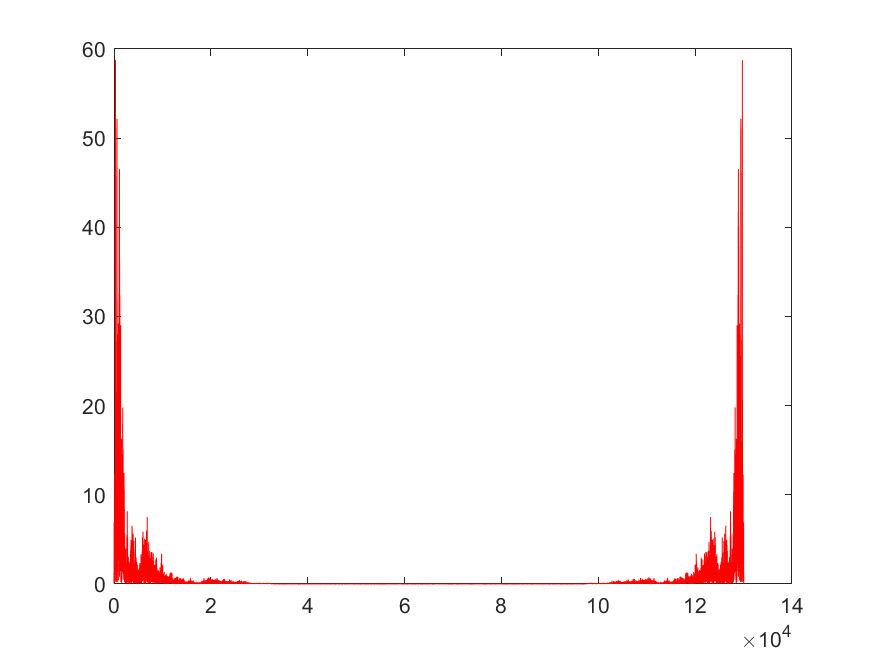
\includegraphics[width = 0.3\textwidth]{problem3/input-freq-Recording1.png}
\label{fig:eff-100}
}
\subfigure{
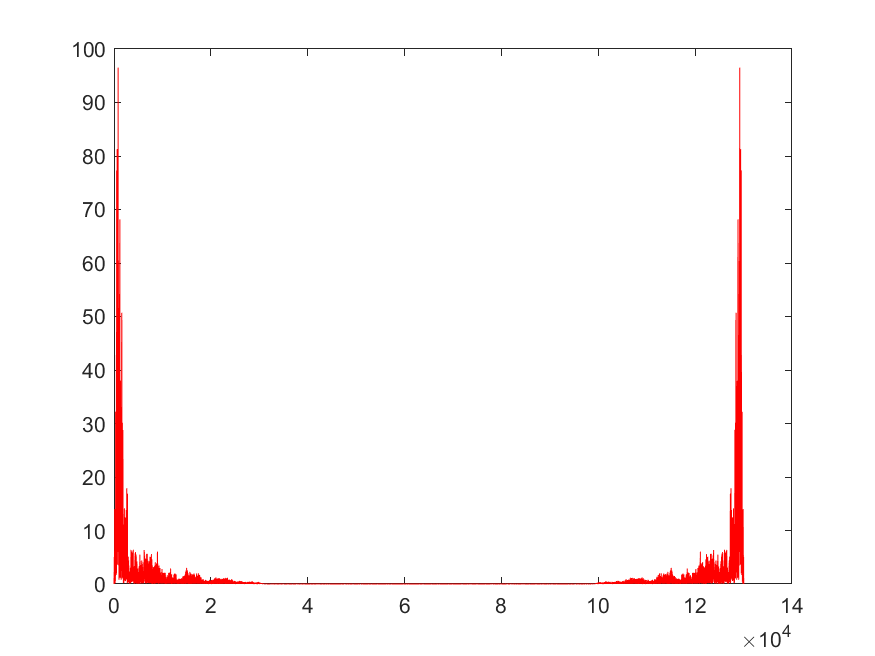
\includegraphics[width = 0.3\textwidth]{problem3/input-freq-Recording2.png}
\label{fig:eff-1000}
}
\subfigure{
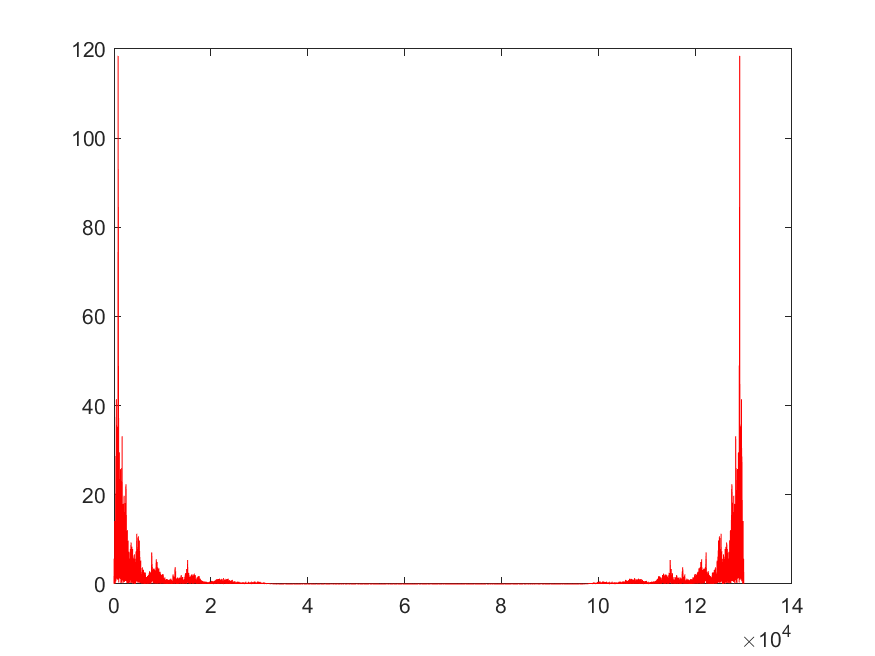
\includegraphics[width = 0.3\textwidth]{problem3/input-freq-Recording3.png}
\label{fig:eff-10000}
}
\caption{原始音频的频域信号}
\label{fig:input-freq}
\end{figure}

之后,截取每个频域信号的前20000个点和后20000个点,在频域上依次排布,得到合成后的频域信号,如图\ref{fig:merge-freq}所示。将得到的频域信号逆变换回时域,便得到合成后的音频。
\begin{figure}[htbp]
\centering
\subfigure[合成后的频域信号]{
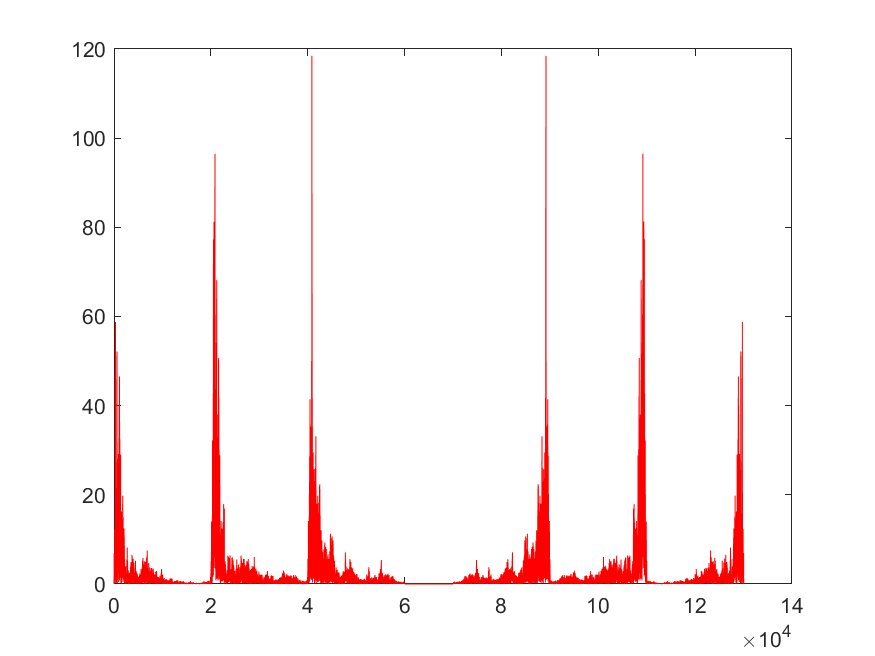
\includegraphics[width = 0.3\textwidth]{problem3/merge-freq.png}
\label{fig:merge-freq}
}
\subfigure[合成音频恢复的频域信号]{
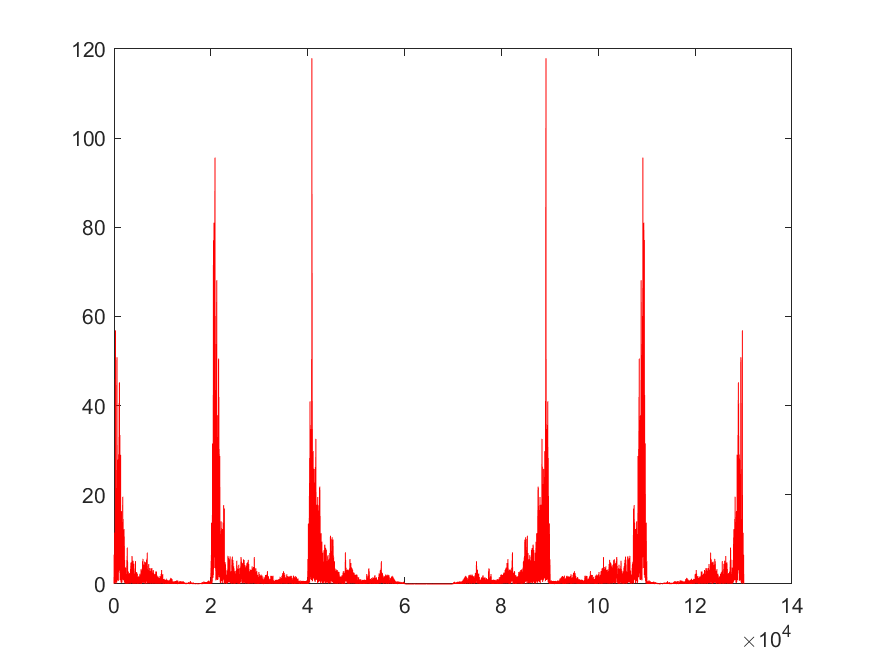
\includegraphics[width = 0.3\textwidth]{problem3/recover-freq-merge.png}
\label{fig:recover-freq}
}
\caption{合成后的频域信号与从合成音频恢复的频域信号}
\end{figure}
\subsubsection{解调过程}
读入合成后的音频,进行傅里叶变换,恢复其频域信号,如图\ref{fig:recover-freq}所示。
将所得的频域信号拆分成3个音频所对饮的频域信号,如图\ref{fig:recover-freq-split}所示。
\begin{figure}[htbp]
\centering
\subfigure{
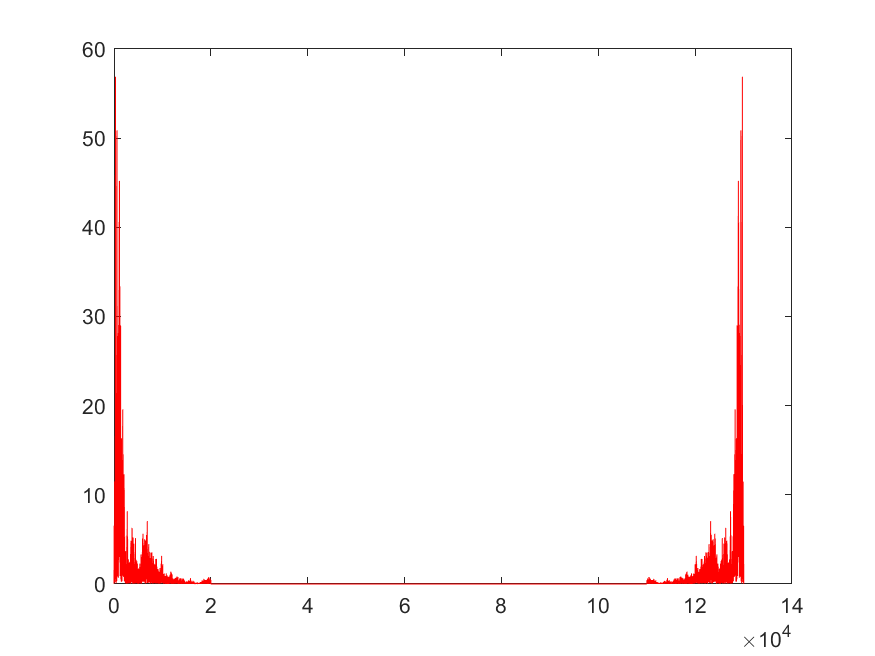
\includegraphics[width = 0.3\textwidth]{problem3/recover-freq-Record1.png}
}
\subfigure{
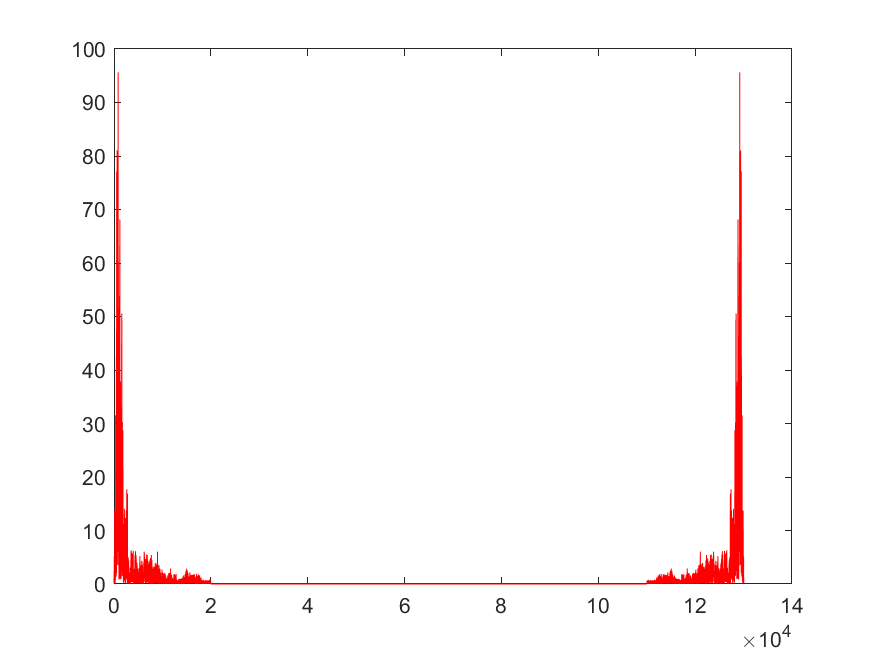
\includegraphics[width = 0.3\textwidth]{problem3/recover-freq-Record2.png}
}
\subfigure{
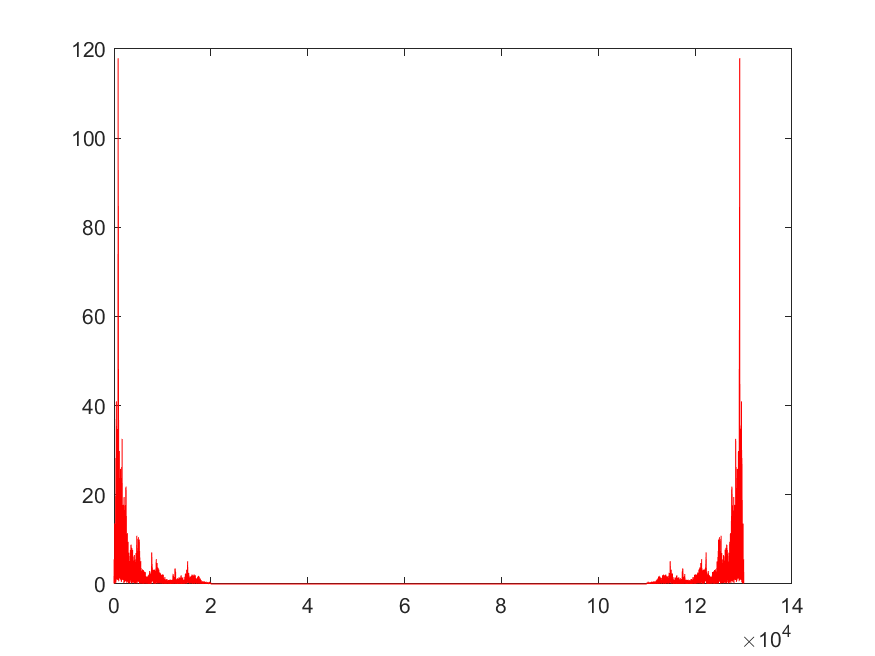
\includegraphics[width = 0.3\textwidth]{problem3/recover-freq-Record3.png}
}
\caption{合成音频拆分后的频域信号}
\label{fig:recover-freq-split}
\end{figure}

之后,对这三个频域信号分别进行傅里叶逆变换,即可得到恢复的时域信号,如图\ref{fig:recover-time}所示。对比图\ref{fig:input-time}可以发现,恢复后的音频几乎没有丢失内容。
\begin{figure}[htbp]
\centering
\subfigure{
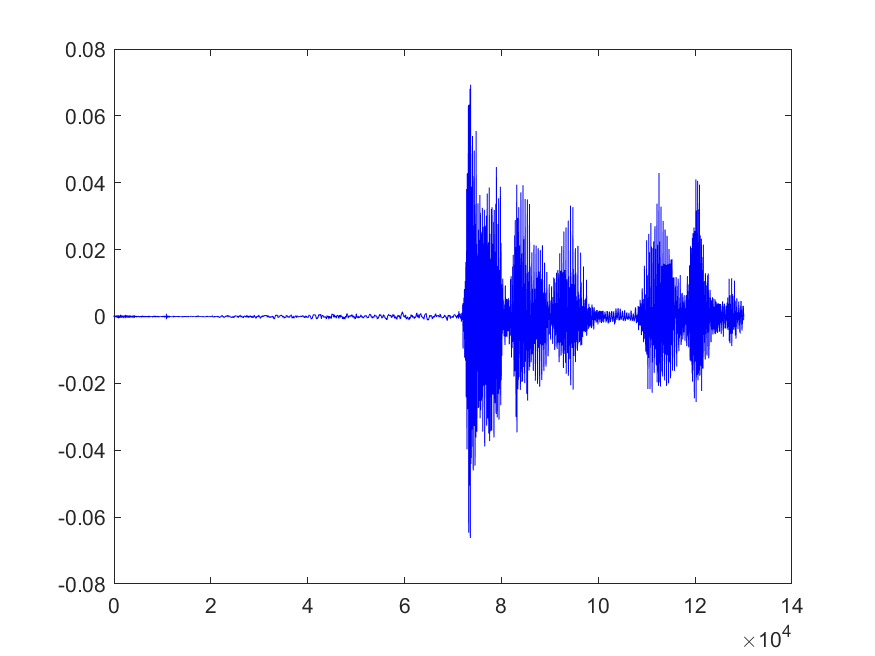
\includegraphics[width = 0.3\textwidth]{problem3/recover-time-Record1.png}
}
\subfigure{
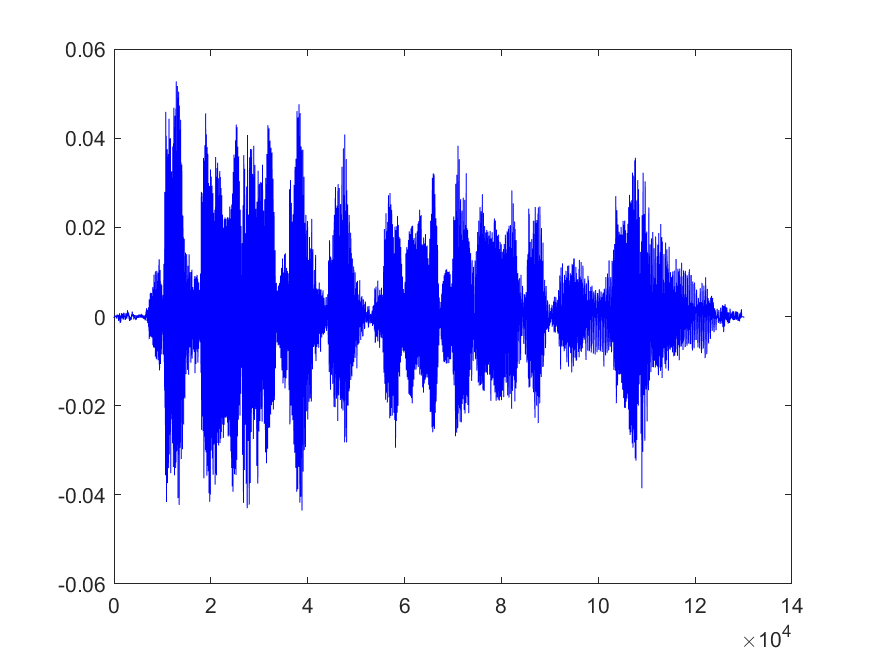
\includegraphics[width = 0.3\textwidth]{problem3/recover-time-Record2.png}
}
\subfigure{
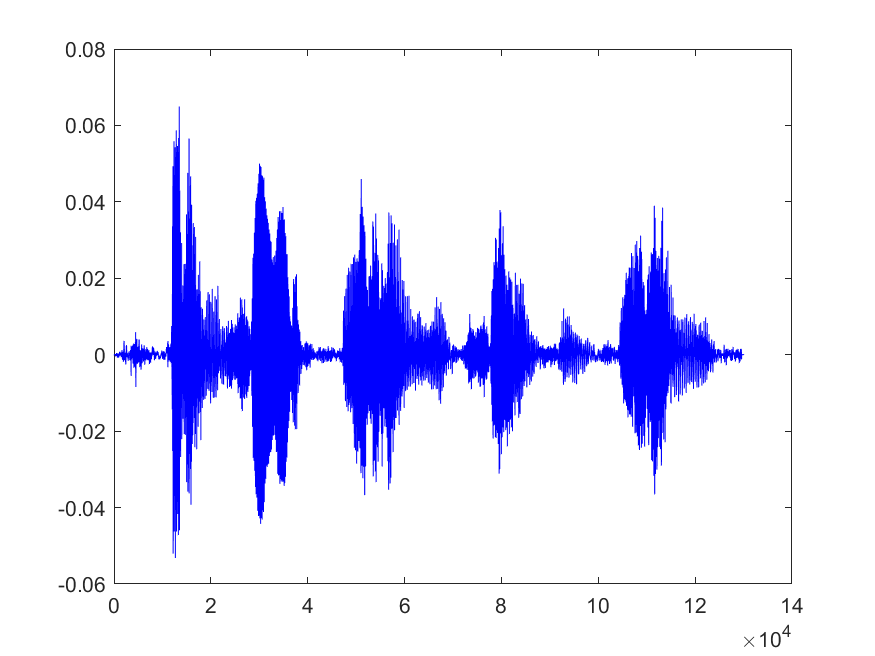
\includegraphics[width = 0.3\textwidth]{problem3/recover-time-Record3.png}
}
\caption{恢复的时域信号}
\label{fig:recover-time}

\end{figure}
\end{document}
